\section{Atomic item access and manipulation}

Both Tensor and TensorArray are iterative. Their dimensions and elements can be efficiently traversed through using looping constructs defined in section \ref{section:loop} in some particularly order. It is sufficient to keep two rules in mind:

\begin{enumerate}
  \item a tensor hold scalars while a tensor array holds fixed-size tensors.
  \item tensor array provides constraint way to encode \textbf{\textit{sparsity}} on the basis of the high-level abstraction tensor.
\end{enumerate}

The second rule helps to make primitives for item access and manipulation supported by TensorArray intelligible: primitives like slice and transpose naturally manipulate items having continous indices will not supported by TensorArray as a first design consideration.

Signatures of operations that access and manipulate tensor and tensor array elements share many similarities.

\begin{tabular}{|c|c|c|}
\hline
&Tensor&TensorArray\\
\hline
index&\checkmark&\checkmark\\
\hline
gather/scatter&\checkmark&\checkmark\\
\hline
slice&\checkmark&\text{\sffamily X}\\
\hline
\end{tabular}

Arithmetic computations defined on tensors and tensor arrays are indexed expressions, therefore iterating over dimensions and accessing items significantly affect performance. Tensor and tensor arrays cannot be efficiently accessed and iterated over by random orders, but in a specific order that will be optimized by program analysis and transformations internally. Figure \ref{mm} shows the intuitioin.

\begin{figure}
\centering
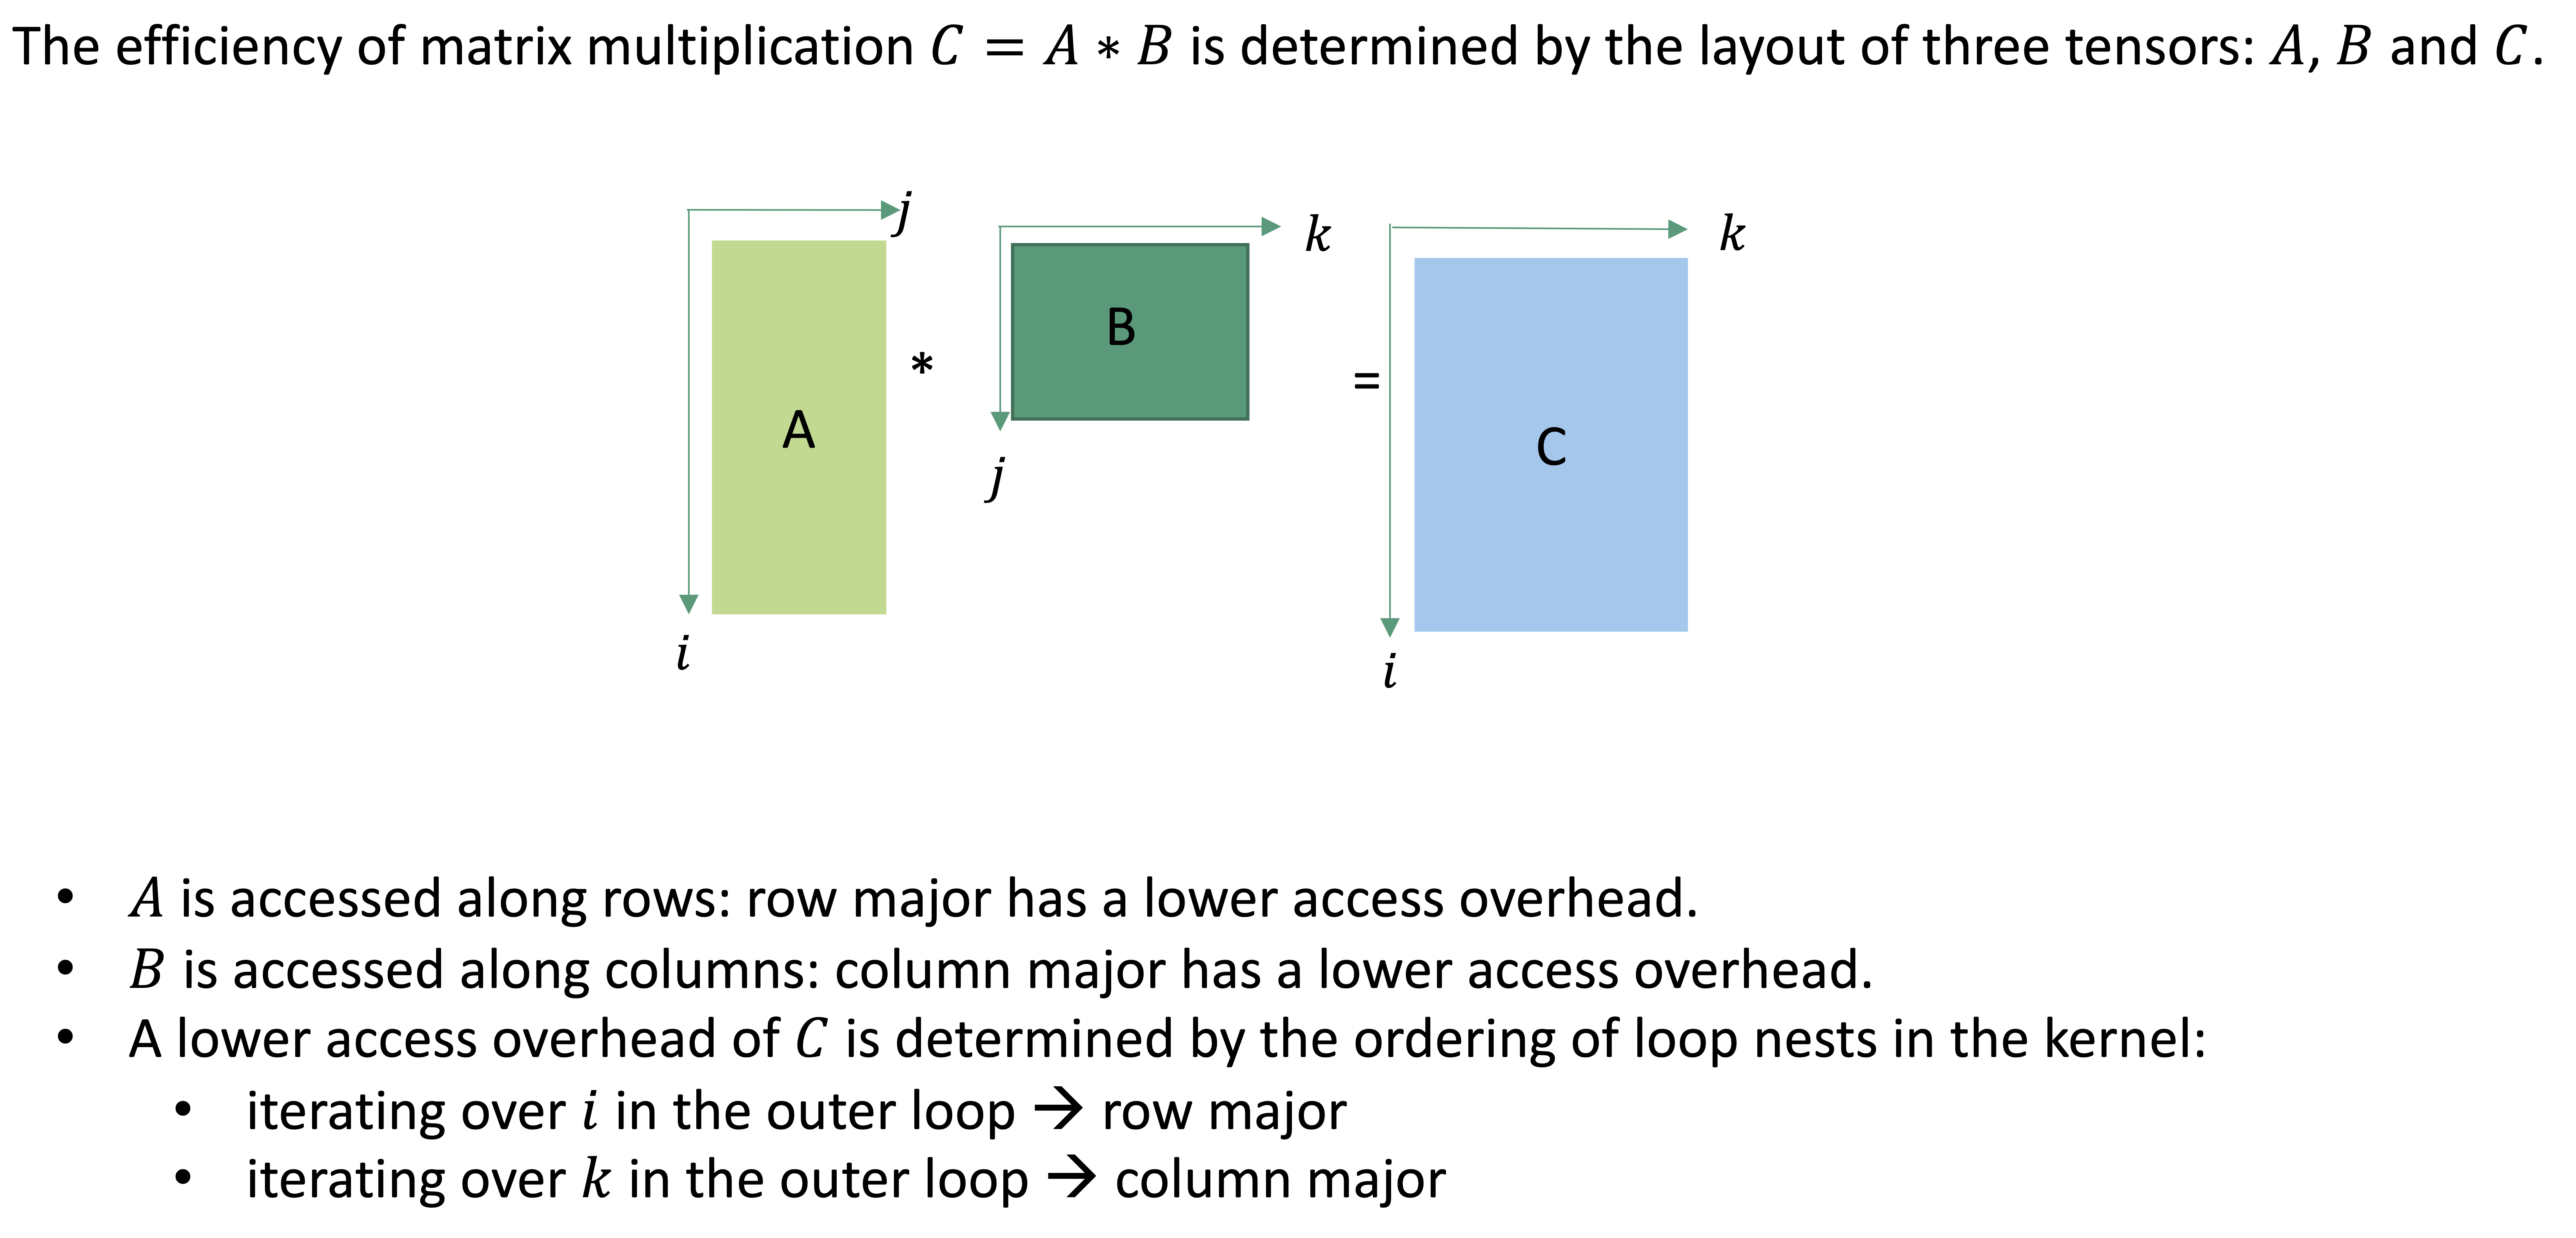
\includegraphics[width=1.\textwidth]{images/mm_example}
\caption{Tensor layout and the order of loops in kernel computations are correlated.}
\label{mm}
\end{figure}

\subsection{\textit{\textbf{index}} and \textit{\textbf{index\_*}}}

\begin{lstlisting}[language=Python]
Y:T = index(func::callable=unary_add, X:Tensor[T], index:Tuple[int])
Y:T = index(func::callable=unary_add, X:TensorArray[T], index:Tuple[int])
\end{lstlisting}

\begin{enumerate}
  \item y = index(x) creates a new Tensor/TensorArray y to hold the result of retrieving a \textbf{\textit{\textcolor{red}{single}}} item from x. Type of the returned result is determined by the elemental type x holds which can be arithmetic type, a fixed-sized tensor, or a tensor array.

  \item index\_* is composite operation
\end{enumerate}

\subsubsection{Shape function}

$S(Y) = S(T)$.

\subsubsection{Forward computation}

a pure access function that maps indices to a single data point.


\subsubsection{Differentiation rule}

\begin{lstlisting}[language=Python]
dx:Tensor[T] = index_add(dX:Tensor[T], dY:T, index:Tuple[int])
\end{lstlisting}

index\_add is a composite operation equivalent to:

\begin{lstlisting}[language=Python]
index(func::callable=add, dX:Tensor[T], dY:T, index:Tuple[int])
\end{lstlisting}

\begin{itemize}
  \item dX is the gradient variable corresponding to X. dX has exactly the same shape as X.
  \item dY is the gradient variable corresponding to Y. dY has exactly the same shape as Y.
  \item The backward computation is to compute dX and dY is known.
\end{itemize}

\subsection{\textit{\textbf{gather\_*}} and \textbf{\textit{scatter\_*}}}

\begin{enumerate}
  \item gather and scatter are dual operations. gather is a multi-index selection method.
  \item \textit{\textbf{gather\_*}} and \textbf{\textit{scatter\_*}} are enssentially composite functions. The "*" part is arithmetic operations, including "max","min","mean","sum".
\end{enumerate}

\begin{lstlisting}[language=Python]
Y:Tensor[T] = gather(func:callable, X:Tensor[T], dim:int, indices:Tuple[int])
Y:Tensor[T] = scatter(func:callable, X:Tensor[T], dim:int, indices:Tuple[int])
\end{lstlisting}

\begin{enumerate}
  \item \textbf{\textit{shape function}}
  \item \textbf{\textit{computation}}
  \item \textbf{\textit{differentiation rule}}
\end{enumerate}


\subsection{\textit{\textbf{slice}} and \textit{\textbf{slice\_*}}}
\begin{lstlisting}[language=Python]
slice(X:Tensor[T], start:int, stride:int, end:int, dim:int) -> Tensor[T]
# or
X[:,idx,:]
\end{lstlisting}

\begin{enumerate}
  \item shape function $S(\mathbf{Y})$

  \begin{equation*}
  \begin{aligned}
    S(\mathbf{Y}) &=\Gamma(S(\mathbf{X}), \text{dim}, \text{keep\_dim}) \\
    &=\left\{
    \begin{aligned}
      &\text{insert}(\text{del}(S(\mathbf{Y}), \text{dim}), \text{dim}, 1)\text{,} \quad \text{if}\quad\text{keep\_dim} \\
      &\text{del}(S(\mathbf{Y}), \text{dim})\text{,} \quad \text{otherwise} \\
    \end{aligned}
    \right. \\
  \end{aligned}
\end{equation*}

\item computation

\item differentiation rule

\end{enumerate}

\section{Layout transformation}

\begin{tabular}{|c|c|c|}
\hline
&Tensor&TensorArray\\
\hline
transpose&\checkmark&\text{\sffamily X}\\
\hline
\end{tabular}


\subsection{\textit{\textbf{transpose}}}

\section{Meta info modification: dimension construction}

\begin{tabular}{|c|c|c|}
\hline
&Tensor&TensorArray\\
\hline
reshape&\checkmark&\text{\sffamily X}\\
\hline
squeeze&\checkmark&\text{\sffamily X}\\
\hline
unsqueeze&\checkmark&\text{\sffamily X}\\
\hline
\end{tabular}

\subsection{\textbf{\textit{reshape}}}
\subsection{\textbf{\textit{squeeze/unsqueeze}}}
